%\documentclass{sig-alternate}
\documentclass[conference]{IEEEtran}

\usepackage{graphicx}
\usepackage{pifont}
\usepackage{url}
\usepackage{code}
\usepackage{amsmath}
\usepackage{algpseudocode} 
\usepackage{algorithmicx}
\usepackage{algorithm}

\newcommand{\comment}[1]{}

\title{Normalizing and Generalizing Test Cases}


\author{\IEEEauthorblockN{%
Alex Groce,\IEEEauthorrefmark{1}
Josie Holmes\IEEEauthorrefmark{2}
Kevin Kellar \IEEEauthorrefmark{3}
}

\IEEEauthorblockA{\IEEEauthorrefmark{1}%
School of Electrical Engineering and Computer Science\\
Oregon State University\\
\IEEEauthorrefmark{2}
Department of Geography\\
Pennsylvania State University
\IEEEauthorrefmark{3}
Crescent Valley High School
}


%\author{\IEEEauthorblockN{Alex Groce, Amin Alipour, Chaoqiang Zhang, Yang Chen, John Regehr}
%\IEEEauthorblockA{School of Electrical Engineering and Computer Science\\
%Oregon State University, Corvallis, OR\\
%Email: agroce@gmail.com, alipourm,zhangch@onid.oregonstate.edu}}
}

\comment{
\numberofauthors{1}
\author{
\alignauthor
Arpit Christi, Matthew Lyle Olson, Mohammad Amin Alipour, Alex Groce\\
\affaddr{School of Electrical Engineering and Computer Science}\\
\affaddr{Oregon State University}
\affaddr{Corvallis, OR USA}\\
%\affaddr{Corvallis, OR}\\
%\affaddr{USA}
}
}

\begin{document}

\maketitle 

\begin{abstract}
Test case reduction has long been seen as essential to effective automated testing.  However, test case reduction simply reduces the \emph{length} of a test case.  It does not attempt to reduce \emph{semantic} complexity.  This paper presents algorithms for normalizing and generalizing test cases.  Rewriting test cases into a \emph{normal form} can reduce semantic complexity and, often, remove steps from an already delta-debugged test case.  Normalization, more importantly, reduces the \emph{number} of test cases that a reader must examine, partially addressing the ``fuzzer taming'' problem of discovering all faults in a large set of failing test cases.  Generalization, in contrast, takes a test case and reports what aspects of the test could have been changed while preserving the property that the test fails.  These algorithms rely on the features of a recently introduced domain-specific language, TSTL.  Normalization plus generalization aids understanding of test cases, including tests for TSTL itself and for complex and widely used Python APIs such as the NumPy numeric computation library and the ArcPy GIS scripting package.  Normalization frequently reduces the number of test cases to be examined by \emph{over an order of magnitude}, and often to just one test case per fault.  Together, ideally, normalization and generalization allow a user to replace reading a large set of test cases that vary in unimportant ways with reading \emph{one annotated test case, summarizing an entire family of similar failures}.
\end{abstract}

\section{Introduction}

It has long been understood that effective automated testing requires
test case reduction \cite{DD,MinUnit,ICSEDiff} to produce test cases
that remove irrelevant operations.  In fact, test case reduction is
now standard practice in industral testing tools such as Mozilla's
{\tt jsfunfuzz}.  However, simply reducing the length of a test case
does not produce any kind of semantic simplicity.  There may be many
1-minimal test cases that present different variations of a single
fault.  In many cases, reading more than one of these test cases
provides no useful additional information on the cause of failure.

Consider the three test cases shown in Figure \ref{threetests}.  These
test cases are obviously very similar, and in fact all lead to a
violation of the property that an AVL tree must always be nearly
balanced, due to a missing call to {\tt rebalance} in {\tt delete} in
a Python implementation of AVL trees.  However, the test cases are
syntactically very different, and a testing system that collects
failing test cases will produce three tests for a user to examine.
While there are methods for attempting to determine which test cases
represent distinct faults \cite{PLDI13}, the ideal solution is
arguably to rewrite all three of these test cases into a single,
normal form that preserves the structure of the failure while removing
such accidental aspects of each test case as the particular integer
values and variables used, and the ordering of assignments and
insertions.

Figure \ref{normalgen} shows the result of applying our \emph{test case
  normalization} method to these three tests, and then applying our
\emph{test case generalization} approach to the normalized test case.
\emph{All three test cases normalize to the same test
case}.  This single test case, in addition to the 10 steps required to produce
the failure, includes comments indicating what about the test case can
be changed while still failing in the same way.  For instance, the
value 1 assigned to {\tt int0} in step 0 is not essential.  It could
be changed to any value in the range 5-20 (the total set of values
allowed by the test generator) without changing the final result.  The
same is true of the assignment of 3 to {\tt int1}.  Similarly, the
exact ordering of many steps in the test case is not important.  Finally,
step 9 is annotated to show that instead of using the existing value
of {\tt int1} (4), a fresh assignment could be inserted before the
{\tt delete} call, setting {\tt
  int1} to 3 instead.  These possible
changes are not meant to be combined --- the annotation claims only
that changing these aspects of the test case one at a time will
preserve failure.

Combining normalization and generalization avoids some common problems
with understanding automatically generated test cases.  For instance,
when a large integer appears in such a test case, the question always
arises --- is this unusual value important, or just a randomly chosen
number of no significance \cite{MakeMost}?  After normalization, any
large values in a test case are sure to be essential, rather than
accidental, because normalization includes value minimization.
Without the additional step of generalization, however, it would be
easy to conclude that \emph{all} small numeric values in normalized tests are
accidental.  Generalization informs a user when a small value is
required to reproduce a failure, and when it is simply an artifact of normalization.

Normalization is not a complete solution to the problem of
identifying distinct faults (one key limitation is that our algorithms do not apply to
complex custom test generators such as CSmith \cite{csmith} or {\tt
  jsfunfuzz} \cite{jsfunfuzz}), but it is highly effective when it applies,
in our experience.
Running 100,000 tests (of length 100) on the faulty AVL tree produces
860 failing test cases with no duplicates.  Normalizing these reduces
the number of distinct failing test cases to only 22.  Of course,
ideally \emph{all} failures due to the same fault would normalize to a
single, representative test case, but we can only aim to approximate
such a canonical form for faults.  Figure \ref{diffnorm} shows a test
case that normalizes differently, and its normalized form (we omit the
generalization, which is not interestingly different than that for the
first normalized test case).

The contributions of this paper are 1) the idea of normalizing and
generalizing test cases, 2) algorithms for normalizing and
generalizing test cases that make use of the abstract graph interface
for testing provided by the TSTL \cite{NFM15,ISSTA15} testing
language, and 3) some initial experimental results showing the value
of test case normalization and generalization.  We show that
normalization and generalization has been key to efforts to understand
complex failing test cases for a widely-used, highly complex library
for GIS automation.

\begin{figure}
{\scriptsize
{\bf Test case \#1}
\begin{code}
avl0 = avl.AVLTree() 
int0 = 4 
int2 = 13 
int3 = 7 
avl0.insert(int2) 
avl0.insert(int3) 
int1 = 15 
avl0.insert(int1) 
avl0.insert(int0) 
avl0.delete(int2)
\end{code}
{\bf Test case \#2}
\begin{code}
int0 = 14 
avl0 = avl.AVLTree() 
int2 = 13 
int1 = 15 
avl0.insert(int1) 
int1 = 11 
avl0.insert(int2) 
avl0.insert(int0) 
avl0.insert(int1) 
avl0.delete(int0) 
\end{code}
{\bf Test case \#3}
\begin{code}
avl1 = avl.AVLTree() 
int3 = 18 
avl1.insert(int3) 
int0 = 5 
int3 = 12 
avl1.insert(int0) 
int0 = 15 
avl1.insert(int0) 
avl1.insert(int3) 
int1 = 15 
avl1.delete(int1) 
\end{code}
}
\caption {Three randomly generated test cases for the same fault.}
\label{threetests}
\end{figure}

\begin{figure}
{\scriptsize
\begin{code}
\textcolor{black!35}{\#[}
int0 = 1                              \textcolor{black!35}{\# STEP 0}
\textcolor{black!35}{\#  or int0 = 5 }
\textcolor{black!35}{\#   - int0 = 20} 
\textcolor{black!35}{\#  swaps with step 4}
int1 = 3                              \textcolor{black!35}{\# STEP 1}
\textcolor{black!35}{\#  or int1 = 5 }
\textcolor{black!35}{\#   - int1 = 20} 
\textcolor{black!35}{\#  swaps with step 6}
avl0 = avl.AVLTree()                  \textcolor{black!35}{\# STEP 2}
\textcolor{black!35}{\#] (steps in [] can be in any order)}
avl0.insert(int0)                     \textcolor{black!35}{\# STEP 3}
\textcolor{black!35}{\#[}
int0 = 2                              \textcolor{black!35}{\# STEP 4}
\textcolor{black!35}{\#  swaps with step 0}
avl0.insert(int1)                     \textcolor{black!35}{\# STEP 5}
\textcolor{black!35}{\#] (steps in [] can be in any order)}
int1 = 4                              \textcolor{black!35}{\# STEP 6}
\textcolor{black!35}{\#  or int1 = 5 }
\textcolor{black!35}{\#   - int1 = 20} 
\textcolor{black!35}{\#  swaps with step 1}
avl0.insert(int1)                     \textcolor{black!35}{\# STEP 7}
avl0.insert(int0)                     \textcolor{black!35}{\# STEP 8}
avl0.delete(int1)                     \textcolor{black!35}{\# STEP 9}
\textcolor{black!35}{\#  or (}
\textcolor{black!35}{\#      int1 = 3  ;}
\textcolor{black!35}{\#      avl0.delete(int1) }
\textcolor{black!35}{\#     )}
\end{code}
}
\caption{Normalization and generalization for all three test cases.
  Lines beginning with \# are comments in Python, used for annotations.}
\label{normalgen}
\end{figure}

\begin{figure}
{\scriptsize
{\bf Test case \#4:}
\begin{code}
int0 = 10 
int2 = 7 
avl1 = avl.AVLTree() 
avl1.insert(int2) 
avl1.insert(int0) 
int1 = 1 
int3 = 1 
avl1.insert(int3) 
int3 = 15 
avl1.insert(int3) 
avl1.delete(int1) 
\end{code}
{\bf Normalized:}
\begin{code}
int0 = 1
int1 = 2
avl0 = avl.AVLTree()
avl0.insert(int0) 
avl0.insert(int1) 
int1 = 3  
avl0.insert(int1) 
int1 = 4  
avl0.insert(int1)  
avl0.delete(int0) 
\end{code}
}
\caption{A differently normalized test case for the same fault}
\label{diffnorm}
\end{figure}

\section{Formal Definitions of Normalization and Generalization}

\subsection{A Brief Introduction to TSTL}

\begin{figure}
{\scriptsize
\begin{code}
@import avl
\vspace{0.05in}
pool: <int> 4 CONST
pool: <avl> 3
\vspace{0.05in}
property: <avl>.check\_balanced()
\vspace{0.05in}
<int> := <[1..20]>
<avl> := avl.AVLTree()
\vspace{0.05in}
<avl>.insert(<int>)
<avl>.delete(<int>)
<avl>.find(<int>)
<avl>.inorder()
\end{code}
}
\caption{Part of a TSTL definition of AVL tree tests.}
\label{fig:example}
\end{figure}

\comment{
\begin{figure}
{\scriptsize
\begin{code}
avl1 = avl.AVLTree()  
int3 = 10  
int1 = 11  
avl1.insert(int1) 
int1 = 1  
avl1.insert(int3) 
avl1.insert(int1) 
int3 = 9  
avl1.insert(int3) 
int2 = 11  
avl1.delete(int2) 
\end{code}
}
\caption{An example TSTL-produced test}
\label{fig:avlrun}
\end{figure}
}

TSTL \cite{NFM15,ISSTA15} is a language for defining the structure of
test cases (usually API-call sequences, but also grammar-based tests using
string construction), and a set of tools for use in generating,
manipulating, and understanding those test cases.  Figure
\ref{fig:example} shows a simplified portion of a TSTL definition of
tests of an AVL tree class, in the latest syntax for TSTL (which
differs slightly from that in the cited papers introducing TSTL).
TSTL provides numerous features not shown in this small example,
including automatic differential testing, complex logging, support for
complex guards, and use of pre- and post- values.  Given a harness
like the one in Figure \ref{fig:example}, TSTL compiles it into a
class file defining an interface for testing that provides features
such as querying the set of available testing actions, restarting a
test, replaying a test, collecting code coverage data, and so forth.
The TSTL release \cite{tstl} provides testing tools that use the
interface for test generation and debugging.

The key point for our purposes is merely that a TSTL test harness
defines a set of \emph{pools} that hold values produced and used
during testing \cite{AndrewsTR} (a common approach to defining
API-testing sequences) and a set of actions that are possible during
testing, typically API calls and assignments to pool values.  In this
example, there are two pools, one named {\tt int} and one named {\tt
  avl}.  There are four instances of the {\tt int} pool, which means
that a test in progress can store up to 4 {\tt int}s at one time (in
variables named {\tt int0}, {\tt int1}, {\tt int2}, and {\tt int3}), and three
instances of the {\tt avl} pool.  The actions defined here are setting
the value of an {\tt int} pool to any integer in the range 1-20
inclusive, setting the value of an {\tt avl} pool to a newly
constructed AVL tree, and calling an AVL tree's {\tt insert}, {\tt
  delete}, {\tt find} and {\tt inorder} methods.  Figure
\ref{threetests} in the introduction shows three
valid test cases produced by running a random test generator on
the TSTL-compiled interface produced by this definition.  TSTL handles
ensuring that tests are well-formed: for example, no pool instance
(such as {\tt avl1} can appear in an action until it has been assigned
a value), and no pool instance that has been assigned a value can be
assigned a different value until it has been used in an action, to
avoid degenerate sequences such as {\tt int3 = 10} followed by {\tt
  int3 = 4}.  Each action in a test case is called a ``step'' --- the
first step of the first test case in Figure \ref{threetests} is storing a new AVL tree in {\tt
  avl0}, for example.

The definition of pools and actions in TSTL defines a \emph{total
  order} on all actions.  First, actions are ordered by their position
in the definition file.  All {\tt insert} actions are therefore before
all {\tt delete} actions, and all {\tt delete} actions are before find
actions.  One line of TSTL typically defines more than one action. For
example, the line of TSTL code {\tt <avl>.insert(<int>)} defines 12 actions, one
for each choice of {\tt avl} and {\tt int} pool instance:  the action set
includes {\tt avl0.insert(int0)}, {\tt avl1.insert(int0)}, {\tt
  avl0.insert(int1)}, and so forth.  These are
ordered lexically, with the first pool appearing in the text taking
precedence ({\tt avl0.insert(int2)} precedes {\tt avl1.insert(int0)},
etc.).  Value ranges such as in the {\tt int} initialization, are also
ordered in the natural way, with lower values first.  Given this total
order, each action can be assigned a unique index, from 0 up to 1 less
than the total number of actions. Initially, this ordering (and
numbering) for each action was intended to allow for a kind of
G\"odel-numbering of tests, for use in proofs about
properties of test-generation algorithms
\cite{AndrewsTR}.  However, it also allows us to concisely define a
practical method for normalizing and generalizing test cases.

In normal TSTL semantics, assigning a
value to the same pool twice in a row is not allowed; until a pool
value is used, it cannot be assigned to again.  However, during
normalization and generalization, this restriction is removed.  The
restriction exists only to prevent the generation of uninteresting
test sequences.  The normalization and generalization algorithms avoid
such sequences by other means, and allowing over-writing assignments
makes normalization much more effective.  Such sequences only appear
in intermediate steps; after normalization, test
cases are guaranteed to not have any remaining sequences invalid in
normal TSTL semantics.

\subsection{Normalization}

A test-case normalization algorithm has a simple goal:  we ideally aim to
produce a function $f : t \rightarrow t$ (a function that takes a test
case and returns a test case) such that:

\begin{enumerate}
\item If $t$ fails, $f(t)$ fails.
\item If $t_1$ and $t_2$ fail due to the same fault, $f(t_1) = f(t_2)$.
\item If $t_1$ and $t_2$ fail due to different faults, $f(t_1) \not=
  f(t_2)$.
\end{enumerate}

Such a function would define a true \emph{canonical form} for test cases, where
each underlying fault is uniquely represented by a single test case.
In general, it seems clear that defining such a function $f$ is (at least) as
difficult as automatic fault localization and repair.  Therefore, we
aim at approximating the goal, by providing a set of simple
transformations such that $f$ changes many tests to the same test, $f$
has
low probability of changing two tests failing for different reasons
into the same test, and $f$ is not unreasonably expensive to compute.
The implementation for $f$ (in fact, for a family of $f$-approximating
functions, with different tradeoffs in runtime and level of
normalization) involves defining a set of rewrite rules such that for a
test $b$ (the base test), the rules define a finite set of candidate
tests $c \in C(b)$, possible simplifications of $b$, where each $c$ is
the result of applying some rewrite, $r_i$ to $b$.  The notion of
simplicity is defined by a restriction on the rewriting rules.  For
any test case $t$, let $R(t)$ be the length of the maximum number of
rewrites that can be applied to $t$, e.g., the longest possible
sequence such that $c_0 = r_{i1}(t), c_1 = r_{i2}(c_0), ... c_n = r_{in}(c_{n-1})$. We
require that $\forall c \in C(b), R(c) < R(b)$.  The number of possible
rewrites for each candidate must be smaller than the number of
possible rewrites for $b$.  This implies further restrictions, e.g., no
rewrite can ever reverse another rewrite's effects.  Such a rewrite
system is \emph{strongly normalizing}:  any sequence of rewrites
chosen will eventually end in a term (test case) that cannot be
further rewritten.

In the setting of TSTL, where test actions have a defined total
order, a simple principle can be applied to produce strongly
normalizing rewrite rules: rewrites should reduce the sum of the
indices of the actions in the test case, or make the test case's
actions more ordered by index.  This approach
provides effective normalization at a significant, but not
impractical, computational cost.

The second principle that determines the rewrite rules is that each
rule should be unlikely to change the underlying cause for test case
failure.  To that end, the rules below always either change at most
one action (possibly in multiple steps, but in a uniform way) or make
\emph{no} changes to the actions performed, only to the pools used or the
positions of actions in the test case.  We cannot guarantee
normalization does not change the underlying fault in a test; however,
the limited scope of rewrites should at least make the likelihood of
fault change (known as ``slippage'' \cite{PLDI13}) around that of
delta-debugging, which is widely accepted as a reasonable tradeoff.

\subsubsection{Definitions and Notation}

In order to formally define normalization, some additional notation is required.
A \emph{step} is an action paired with an index indicating its
position in a test case,
where the first action is step 0, etc.; e.g., $(2: a)$ indicates the
third step of the test is action $a$ (indexing is from 0). 
$\Delta(t,t')$ is the set of all steps in $t$ such that $t(i) \not= t'(i)$.

We use the $<$ operator over various types:
$a < b$ iff the index of action $a$ is lower
than that of action $b$.  We compare steps with $<$ by comparing their
actions --- $(i,a) < (j,b)$ iff $a < b$.  For a set or sequence of actions or steps, we define the $min$ of the
set to be the lowest indexed action in the set, and use
these to compare sets:  $s_1 < s_2$ iff $min(s_1) < min(s_2)$. For pools,
$p < p'$ if and only if $p$'s index is lower than the index for $p'$
\emph{and} $p$ and $p'$ are from the same pool.

The rewrite $t[x \Rightarrow y]$ denotes the test t with all instances of $x$
replaced by $y$.  Here, $x$ and $y$ can be actions, steps, or pools.
$t[x \Leftrightarrow y]$ is similar, except that $x$ and $y$ are
swapped.  Rewrite $t(i,j)[x \Rightarrow y]$ is the same as $t[x \Rightarrow
y]$, except that the replacement is only applied between steps $i$ and
$j$, inclusive.  Finally, $t_i(x)$ denotes $t$ with all steps
containing $x$ that are before step $i$ moved to step $i$, preserving
their previous order, and moving steps at $i$ and after $i$ to make room.

\subsubsection{Rewrite Rules}

\begin{enumerate}
\item {\bf SimplifyAll:}
$c = b[a \Rightarrow a']$\\
\-\ \ \ \emph{where} $a' < a$\\
Covers the case where all appearances of an action can be replaced with a 
simpler (lower-indexed) action. 
\item {\bf ReplacePool:}
$c = b(i,j)[p \Rightarrow p']$\\ 
\-\ \ \ \emph{where} $p < p'$ and $0 \leq i < j <
|b|$\\
Covers the case when all appearances of an instance of a pool can be replaced with 
a lower-indexed instance of that pool (with possible restriction to a range of steps).
\item {\bf ReplaceMovePool:}
$c = b_{\rightarrow i}(p')[p \Rightarrow p']$\\
\-\ \ \ \emph{where} $p < p'$ and $0
\leq i < |b|$\\
Covers the case when all appearances of an instance of a pool can be replaced with
a lower-indexed instance of that pool, if all assignments to the new instance before a
certain step are moved to that step.
\item {\bf SimplifySingle:}
$c = b[(i: a) \Rightarrow (i: a')]$\\
\-\ \ \ \emph{where} $a' < a$\\
Covers the case where one action can be replaced with a 
simpler (lower-indexed) action. 
\item {\bf SwapPool:}
$c = b(i,j)[p \Leftrightarrow p']$\\
\-\ \ \ \emph{where} $\Delta(c,b) < \Delta(b,c)$\\
\-\ \ \ and $0 \leq i < j < |b|$\\
\-\ \ \ and $p < p'$\\
Covers the case where swapping two pool instances (within a range of steps) reduces
the minimal action index of the modified steps.
\item {\bf SwapAction:}
$c = b[(i: a) \Rightarrow (i: b), (j: b) \Rightarrow (j: a)]$\\
\-\ \ \ \emph{where} $i < j$ and
$b < a$\\
Covers the case where two actions can be swapped in the test, with the
lower-indexed action now appearing earlier.
\item {\bf ReduceAction:}
$c = b[(i: a) \Rightarrow (i: a')]$\\
\-\ \ \ \emph{where} $|ddmin(c)| < |ddmin(b)|$\\
Covers the case where an action can be replaced by any action (not just lower-indexed
actions) and this enables further delta-debugging-based reduction of
the test case's length.
\end{enumerate}

\subsubsection{Normalization Algorithm}

These rules alone do not determine a complete normalization method; it is
also required to determine an order in which they are applied.  The
order in our default implementation is the order above, with the
modification that in practice the {\bf ReplacePool} and {\bf
  ReplaceMovePool} rewrites are both performed at once, interleaved
(e.g., for every possible replacement of a pool, both rules are
checked, in the order given above).  The core algorithm, given a set
of ordered rewrite rules defining $C(b)$ is given as Algorithm
\ref{simpalg}.  Here {\tt pred} is an arbitrary predicate indicating
that the candidate test still satisfies the property of interest that
held for the original test $b$.  In most cases, this predicate will be
``the test fails'' but we also have preserved
code coverage for regression suites \cite{icst2014}.  Notice that
after applying each rewrite rule, we perform delta-debugging on the
new base test case, since often a rewrite makes other steps irrelevant.

\begin{algorithm}
\caption{Basic algorithm for normalization}
\label{simpalg}
\begin{algorithmic}[1]
\State {modified = True}
\While {modified}
\State {modified = False}
\For {$c \in C(b)$}
\If{pred($c$)}
\State modified = True 
\State $b$ = $ddmin(c)$
\State {\bf break} (exit {\bf for} loop) 
\EndIf 
\EndFor 
\EndWhile 
\State return $b$
\end{algorithmic}
\end{algorithm}

Assume there are $k$ steps in the test case and $n$ possible actions.
We approximate the complexity of normalization by first bounding the cost for each pass through the
inner {\bf for} loop.  The action replacements and pool movement
replacement rewrites (1, 3, 4, and 7) all require at most $k (n-1)$
predicate checks when no simplification takes place, and all checks
fail.  The {\bf SwapAction} rewrite can obviously require no more than
$k^2$ checks, and the {\bf ReplacePool} rewrite fewer than
$k^2 (n-1)$\footnote{The details of how these bounds are determined,
  in that pool changes are also action changes, are not critical, and
  a more detailed analysis is somewhat involved, and beyond the scope
  of this paper; we note that like delta-debugging, the worst-case
  complexity is seldom observed, and offer some further optimizations
  below.}.  Therefore each inner loop run requires at most
$k^2 + k^2(n-1) + 4k(n-1)$ checks (we assume a constant cost to run a
check --- unlike in delta-debugging, this is a reasonable assumption, as few
rules change the length of the test).  Each time the inner loop finds
a valid rewrite, there is also the cost of a delta-debugging step,
which is at worst quadratic in $k$ \cite{DD}.  The cost of the inner
loop is therefore $O(k^2n)$.  How many times can this inner loop run
(e.g., how many times can the {\bf while} loop run)?  Each
action can be replaced fewer than $n$ times, since each
replacement (or at least one replacement in each rewrite,
for the pool changes) must decrease the index of the action.  Steps
can be swapped fewer than $k$ times, obviously.  Each  {\bf
  ReduceAction} rewrite requires reducing the length of the
test, giving it a total (not per-step, like the other bounds) bound of
$k$ successful rewrites.  This gives us an upper bound of $kn +
k^2 + k$ executions for the outer loop, and a total runtime that is
$O(k^4n)$.

In practice, most actions are not enabled at most steps, and
the rules are applied in an order that quickly converges on a normal
form for many test cases.  In our experiments, normalization is only
very expensive when delta-debugging is also costly, and appears to be
worse than delta-debugging by a constant factor, somewhere in the
range of 2-10x, usually closer to 10x.  We believe that if
normalization can decrease human effort in examining large numbers of
redundant test cases, this price is more than reasonable.  Measuring
the payoff from improved understanding of test cases is difficult;
however, in multiple fault settings, we hope normalization can often
provide a quantifiable value in shorter time until all faults have
been examined by a human, for bug triage \cite{PLDI13}.

\subsubsection{Normalization Optimizations}

The simplest and most important optimization is to improve on the
constant ordering of rewrite rules.  In our implementation, once a
rule fails to produce a candidate that satisfies {\tt pred} that rule
is moved to the end of the ordering of rewrites.  This optimization
followed the observation that almost always once a rule fails to
produce any changes in a test case, it never applies again.  This
simple change, in our experience, typically halves the time required
for normalization.

For test cases with a very short runtime, this algorithm (with
reordering) is usually practical: though more expensive than delta-debugging
it still requires  less than a minute to run.  However, when test case
execution is expensive, the set of candidate test cases must be
further restricted.  In our experiments, we found that restricting
action replacements to cases where the Levenshtein \cite{Lev} distance
(text edit distance) between the code for the actions was bounded was effective in reducing runtime, while almost always having no
impact on the final result.  In practice, most test actions can only
be replaced by syntactically similar actions, without completely
changing test semantics.

A further useful optimization when normalizing large numbers of tests
of the same SUT is to cache results, so that as soon as the rewrite
sequence produces a previously seen test, the final result can be
returned (since the algorithm is deterministic).   For very large
numbers of tests, this is the most important optimization.
Interestingly, though it is also deterministic, caching
delta-debugging results is almost useless, since the chance of seeing
an exact match is very small; this is true with the initial input to
normalization, but a few pool and value changes often result in a
cache hit. For systems with
very expensive replay, the delta-debugging of each new base test case
can also be omitted, as we can count on the {\bf ReduceAction} rewrite to
eventually remove useless steps (however, this may come at a cost of
attempts to rewrite steps that could be removed).

Finally, it is easy to parallelize the normalization of a test case by
checking the predicate over multiple candidates at once.  As soon as a
candidate satisfies the predicate, one of two options are available:
either the normalization can proceed with that candidate as the new
base, making the algorithm nondeterministic (in theory; in
practice we suspect the same final result will usually appear), or the
algorithm can wait for all earlier-in-sequence candidates to be
checked, and only proceed when no candidate that would be checked
first in the sequential version of the algorithm is in the work
queue.

\subsection{Normalization Example}
\label{formalexample}

\begin{figure}
{\scriptsize
{\bf Original test case:}
\begin{code}
  0: int0 = 10 
  1: int2 = 7 
  2: avl1 = avl.AVLTree() 
  3: avl1.insert(int2) 
  4: avl1.insert(int0) 
  5: int1 = 1 
  6: int3 = 1 
  7: avl1.insert(int3) 
  8: int3 = 15 
  9: avl1.insert(int3) 
 10: avl1.delete(int1) 
\end{code}
{\bf Normalization Steps:}
\begin{code}
{\bf SimplifyAll}: int0 = 10 $\Rightarrow$ int0 = 2 
{\bf SimplifyAll}: int2 = 7  $\Rightarrow$ int2 = 3 
{\bf SimplifyAll}: int3 = 15  $\Rightarrow$ int3 = 4 
{\bf ReplacePool}: int2 $\Rightarrow$ int1
{\bf ReplacePool}: avl1 $\Rightarrow$ avl0
{\bf ReplacePool}: int3 $\Rightarrow$ int0
{\bf SwapAction}: (0: int0 = 2)  $\Leftrightarrow$ (6: int0 = 1)
{\bf SwapPool}: int0 $\Leftrightarrow$ int1 (between steps 2 and 10)
{\bf SwapAction}: (1: int1 = 3)  $\Rightarrow$ (5: int1 = 2)
\end{code}
{\bf Normalized:}
\begin{code}
  0: int0 = 1
  1: int1 = 2
  2: avl0 = avl.AVLTree()
  3: avl0.insert(int0) 
  4: avl0.insert(int1) 
  5: int1 = 3  
  6: avl0.insert(int1) 
  7: int1 = 4  
  8: avl0.insert(int1)  
  9: avl0.delete(int0) 
\end{code}
}
\caption{An example of normalization steps.}
\label{diffnorm}
\end{figure}

Figure \ref{diffnorm} shows the sequence of successful rewrites in
normalizing a simple AVL tree test failure.  Note that the numbering
of steps appears inconsistent in the first {\bf SwapAction} because a
successful delta-debugging removes a no-longer-needed step after a
rewrite.  In our experience, this pattern, where successful rewrites
are roughly equal to the original number of steps, is frequent across SUTs.

\subsection{Generalization}

\subsubsection{Generalization Algorithm}

The core idea of generalization is to use methods similar to those
involved in normalization to provide a user with information about
changeable aspects of a test case.  Some values and orderings of steps
in a test case are \emph{essential} to the failure: when changed, they
cause the test case to no longer fail.  Many others, however, are
\emph{accidental} --- any concrete test case has to choose \emph{some}
values and step ordering (for us, that enforced by the normalization
process) but many such choices are arbitrary, or at least allow
variance, with respect to the cause of failure.  Generalization
performs experiments to distinguish essential and accidental aspects
of a test case, and summarizes the results.  The core algorithm
(Algorithm \ref{genalg}) is simple.

\begin{algorithm}
\caption{Basic algorithm for generalization}
\label{genalg}
\begin{algorithmic}[1]
\State {swap = $\emptyset$}
\State {replace = $\emptyset$}
\For {$(i, a) \in t$}
\For {$a' : a' > a$}:
\If {pred($t[(i,a) \Rightarrow (i,a')]$)}
\State replace = replace $\cup ((i,a),(i,a'))$
\EndIf
\EndFor 
\For{$j : i < j < |t|-1 \wedge (j: b) > (i: a) $}
\If {pred($t[(i: a) \Rightarrow (i: b), (j: b) \Rightarrow (j: a)]$)}
\State swap = swap $\cup ((i,a),(j,b))$
\EndIf
\EndFor
\EndFor
\State {return (swap, replace)}
\end{algorithmic}
\end{algorithm}

This algorithm collects all steps that can be replaced with other
actions or swapped with other steps, and returns the set to be
reported to the user.  This version assumes the test has already been
normalized, but can be extended to any test case by removing the
restrictions that $a > a'$ and $(j : b) > (i : a)$.  The complexity of
generalization is simpler to determine than that of normalization: if
we assume all actions are enabled at each step, and there are $n$
actions and $k$ steps, checking for replacements requires $k (n-1)$
test case executions (when every action is the lowest-indexed action).
In that worst case, no swaps are possible.  The complexity of checking
for swaps in the worst case is quadratic in $k$.  In practice, most
actions are not enabled at most steps, and most actions in a test case
are not the lowest-indexed action.  Basic generalization is trivial to
parallelize, as all checks are independent.


\subsubsection{Fresh Values and Misleading Test Cases}
\label{freshgen}

A side-effect of delta-debugging and of normalization is the reduction
of the number of variables used in a test case.  While usually helpful
for understanding, this can sometimes result in misleading test
cases.  In a stateful system, putting the system into a bad state may require
building a complex object.  Once system state is corrupted, however,
the complex object is irrelevant, and its appearance in the call
leading to failure can be misleading.  In previous work at NASA, we
observed that sometimes a delta-debugged file system test case
\cite{ICSEDiff,AMAI} would use an open file descriptor in a call,
leading to the suspicion that the file had been corrupted, when in
fact the file system's state in memory was damaged, and the same
operation on any file would produce the same problem.  To address this
problem, we present a more aggressive generalization than
replacement and swap:  replacing a pool use with a
fresh value.  

As an example, consider the test case in Figure \ref{fig:mislead},
produced by our TSTL harness that uses TSTL to test TSTL
itself\footnote{Since TSTL provides a Python API, that API can be used
  as the SUT in testing; we have discovered several important TSTL
  bugs this way.}.  The problem involves an invalid normalization
cache, produced by normalizing a test with only one action.  Without
generalization, it appears that the failure comes when this test is
normalized a second time.  However, the information after step 6 shows
that in fact the failure will take place even if a newly created empty test is
normalized.  Without this generalization, the state of the {\tt test} pool
may appear to be important, not the state of the TSTL system itself.

\begin{figure}
{\scriptsize
\begin{code}
\textcolor{black!45}{\#[}
test0 = []                             \textcolor{black!45}{\# STEP 0}
\textcolor{black!45}{\#  or test0 = sut0.test() }
actionlist0 = sut0.actions()           \textcolor{black!45}{\# STEP 1}
\textcolor{black!45}{\#  or actionlist0 = sut0.enabled() }
\textcolor{black!45}{\#] (steps in [] can be in any order)}
action0 = actionlist0[0]               \textcolor{black!45}{\# STEP 2}
\textcolor{black!45}{\#[}
test0.append(action0)                  \textcolor{black!45}{\# STEP 3}
pred0 = sut0.fails                     \textcolor{black!45}{\# STEP 4}
\textcolor{black!45}{\#] (steps in [] can be in any order)}
sut0.normalize(test0,pred0)            \textcolor{black!45}{\# STEP 5}
sut0.normalize(test0,pred0)            \textcolor{black!45}{\# STEP 6}
\textcolor{black!45}{\#  or (}
\textcolor{black!45}{\#      test0 = []  ;}
\textcolor{black!45}{\#      sut0.normalize(test0,pred0) }
\textcolor{black!45}{\#     )}
\end{code}
}
\caption{Generalized test for TSTL itself, showing fresh-object
  generalization.}
\label{fig:mislead}
\end{figure}

Formalizing this generalization requires some additional notation.
$U(a)$ provides a list of pools \emph{used} in the action $a$ --- pools that
appear in the action, not on the left-hand side of an assignment.
$I(a,p)$ is a predicate that is true iff action $a$ stores a new value
in pool $p$.  Finally, $t[+(a: i)]$ denotes test $t$ with the action
$a$ inserted at step $i$ and each step from $i$ onwards moved to a
position one higher.

\begin{algorithm}
\caption{Basic algorithm for fresh object generalization}
\label{freshalg}
\begin{algorithmic}[1]
\State {fresh = $\emptyset$}
\For {$(i, a) \in t$}
\For{$p \in U(a)$}
\For{$a' : I(a',p)$}
\If {pred($t[+(a',i)]$)}
\State fresh = fresh $\cup (i,a')$
\EndIf
\EndFor 
\EndFor
\EndFor
\State {return fresh}
\end{algorithmic}
\end{algorithm}

In practice, the {\tt fresh} set returned should be pruned to avoid
redundant actions.  It is not useful information that the sequence {\tt
  int0 = 1 ; int1 = 2; int0 = 1; f(int0)} fails if {\tt int0 = 1; int1
  = 2; f(int0)} fails.  Redundancy elimination also needs to take into
account the potential assignments to a pool from the {\tt replace}
generalization, which are also redundant.  Furthermore, it is useful
to distinguish between pools that are never modified, only assigned
to, and pools that are modified without appearing on a left-hand
side.  As an example, if an integer is used as an argument to a
function, the pool value's last assignment is still valid and should
be omitted from ``fresh'' values, as redundant.  However, calling a
function on an AVL tree or a list may modify the object, making an
assignment non-redundant, even if it is the last appearance of that
pool as lhs.  Further extensions of the fresh value generalization
could be considered; e.g., if a fresh value for some object requires use
of a complex constructor, the values required to call the constructor
could also be produced, if they do not appear in the test case
previously (if only one of a set of constructors can produce a fresh
value that will satisfy the predicate).  However, in our experiments
so far, simple fresh value generation suffices, since the needed
inputs to constructors are usually available in pools, and it is not
important to know \emph{all} constructor inputs that could result in a
successful fresh value generalization.

\subsection{Discussion}

TSTL's conversion of testing into a
graph exploration problem \cite{NFM15}, where a test generation
algorithm can be agnostic as to the underlying SUT, or even the
language of the system under test, enables us to produce semantic
normalization and generalization by simple syntactic means.  The current TSTL implementation is
in Python\footnote{There is also a beta Java version, with a
  simpler version of normalization.}, but the
normalization and generalization algorithms do not depend on the
underlying language, only on the abstract notions of actions and
pools.


\section {Experimental Results}

This section presents some initial results of applying normalization
and generalization.  All tests were generated using pure random testing,
based on TSTL harnesses developed previously, all included in the
TSTL release \cite{tstl}.  We also tested the
Python interface to Z3 \cite{z3}, but did not find faults thus far;
normalization did help produce more comprehensible and uniform Z3
quick tests \cite{icst2014}.

These experiments are not intended to provide a full evaluation of
normalization and generalization, but to establish the basic potential
value of
the techniques, and some initial data on core research questions, over
seven Python libraries ranging from small to large and complex.
These are:
{\bf RQ1:} How effectively does normalization reduce the number of
failures reported? {\bf RQ2:} How often does normalization lose
faults? {\bf RQ3:} What is the cost of normalization and generalization? {\bf RQ4:} How
much additional reduction over delta-debugging can normalization
provide? We also examined the question of whether normalization and generalization provide
substantial benefits in understanding complex tests, in a qualitative
way, by examining tests for some of the larger SUTs studied.
The primary
threat to validity is that we have only applied our methods  to tests produced using random testing for 
seven subjects, written in Python (some small, some large).  The
benefits for human understanding would require a human study to fully evaluate.

Our experimental subjects and results can be divided into three parts.  First, we studied simple programs
with small failing tests, in order to use mutation analysis to
thoroughly investigate {\bf RQ1-3}, especially in the context of tests
without a good fault signature, where normalization is most needed to
reduce failures to examine.  Second, we studied
larger and more realistic programs with a large number of lengthy,
complex failures, largely
to provide more information on {\bf RQ4} (additional reduction beyond
that provided by delta-debugging).  Finally, we examined a much smaller
number of failures for subjects where each reduction or normalization
required an extremely long time to complete, and understanding
individual tests is a difficult task.

\subsection{Mutation-Based Experiments}

%\subsubsection{AVLTree}

Our small subjects are a
simple Python AVL tree found on the web
\cite{avltree}, with 225 lines of code\footnote{All sizes non-comment,
  non-blank lines, by cloc \cite{cloc}.} and a
simple XML parser with about 260 lines of code \cite{myxml}.  For both
subjects, we produced mutants \cite{mutant} using the MutPy tool
\cite{mutpy}, then filtered the set to contain only mutants that produced
at least 1 failing test in 1,000 tests.  We then used the filtered
mutants to generate higher-order mutants (``pairs'') composed of two mutants,
such that each of the mutants could be detected in isolation:  that
is, there existed at least one failing test such that fixing the other
mutant left the test still failing.  For AVL, there were 82 failing
mutants (out of 228 total), from which we sampled 364 pairs
(restricted to mutants modifying different source lines).  Of these,
238 pairs had independently detectable faults.  For XML, only 5 of 357
mutants generated were detectable due to a weak specification.  There were 9 pairs with independently
detectable faults.

\subsubsection{RQ1: Reduction in number of failures}

\begin{figure}
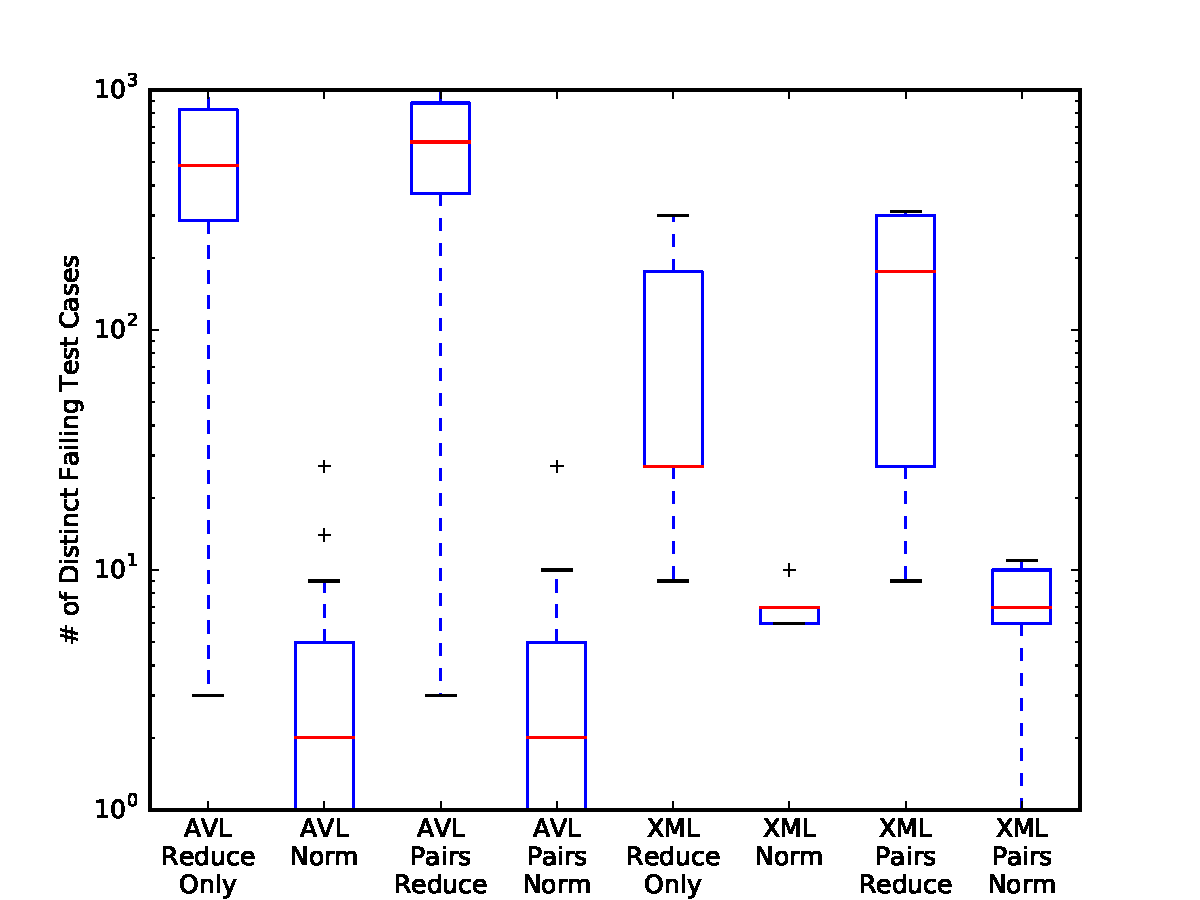
\includegraphics[width=\columnwidth]{length}
\caption{Effects of normalization on AVLTree and XML parser mutants.}
\label{normeffect}
\end{figure}

Figure \ref{normeffect} shows the reduction in number of distinct
failing tests produced by reduction alone vs. reduction and
normalization, for AVLTree and XML mutants; note the
log-scale y-axis.  All
differences are statistically significant by paired Wilcoxon test \cite{arcuri2014hitchhiker}, at $p
< 0.05$.  For 38 of the 82 AVL single mutants, normalization was
perfect (1 failure); for XML, only one mutant was perfectly
normalized.  Normalization was perfect (1 or 2 failures\footnote{Yes,
  in some cases, a single test case detects either fault unless both
  are fixed.}) for 115 of the 238 AVLTree pairs, but none of the XML
pairs.  Even when the improvement was perfect, it was usually quite dramatic, from about 500 failures on average per mutant or
mutant pair for AVL and about
100 for XML to less than 5 for AVL and less than 10 for XML.

A second way to examine reduction in a multi-fault setting is to
consider the mean number of tests a user must examine before seeing
all faults \cite{PLDI13}.  For the AVL mutant pairs, a user must
examine almost 20 tests (on average) before encountering at least
one instance of both faults.  With normalization, this  drops
to a mean of just 2 tests.  The difference is significant with
$p\leq1.4\times10^{-6}$.  The
difference in number of tests before encountering both faults in XML pairs
was not statistically significant (for these 5 faults,
failure rates are very similar, so hitting both is easy no matter how
many failures there are; however, satisfying oneself that all faults
have been seen is much harder with a very large number of tests to examine). 

\subsubsection{RQ2: Slippage via normalization}

Mutants also provided a way to evaluate the danger of
normalization losing faults, {\bf RQ2}.  Faults can be lost when normalization
changes a test failing due to one fault into a test failing
due to a different fault, a problem known as ``slippage''
\cite{PLDI13,slippage}.  The AVL and XML testers pose an interesting
slippage challenge, as the failure signatures are not useful, and the tests
for faults are likely to be very close to each other in the
combinatorial space, due to the simplicity of the tested interfaces.
Out of the 238 AVL mutant pairs, normalization produced tests
exposing both faults for 80.7\% of pairs (19.3\% slippage at the
suite level).  Interestingly, for 4 AVLTree pairs
normalization took a set of reduced tests not capable of exposing
both faults, and produced a smaller set of tests that \emph{was} capable
of detecting both faults.  For XML pairs, the slippage rate was 12.5\%
(of the 9 pairs, only 1 lost a fault, and in that case the faults were
both syntactically and semantically very similar: within 1 line and
with similar effects).

Recall that of our 364 AVL mutant pairs, only 238 could be
independently detected; in most cases this was due to reduction itself
introducing slippage (in a few cases, one fault completely masks
another; e.g., if the constructor always fails, {\tt insert} failures
cannot be detected).  Slippage due to reduction itself is very rare for some SUTs but common
for others (up to 23\% for Mozilla's JavaScript engine)
\cite{PLDI13}.  For the AVLTree example, the slippage rate for
reduction is almost 30\%, 10\% \emph{worse} than that for
normalization; for XML, however, reduction alone never caused slippage.  Mitigation
approaches for slippage during reduction \cite{slippage} should also
apply to normalization.

\subsubsection{RQ3: Normalization runtime}

The mean cost to reduce an AVLTree test was 0.05 seconds; the mean cost for normalization was 0.38
seconds.   For XML, the mean cost for reduction was 12.6 seconds vs.
120.8 seconds for normalization.  Note that in all our results the cost of normalization is given on an
already-reduced test, so the inputs for normalization are smaller than
those for reduction; however, this is the expected use-case for
normalization.  Comparing on equal-sized tests would simply involve
adding the costs for reduction to those for normalization, as an
additional step of normalization.  The criticality of caching
for normalizing large numbers of tests is evident.  Out of 60,226
normalizations performed in our full AVLTree mutant experiments,
59,972 (99.6\%) resulted in a cache hit (most of these after a small
number of normalization steps).  In fact, the total number of rewrites
performed during the AVL mutant experiments was only 145,780, for a mean of only
2.4 non-cache-hit rewrites of each test.  For XML, there were 3,829 cache hits over
a total of 3,929 normalizations.

\mycomment{ 

a set of 82 mutants \cite{mutant} of AVLTree
\cite{Hunter:2007} ({\bf RQ1}).  Of the 228 mutants produced by MutPy
\cite{mutpy}, only these 82 produced at least 1 failure in 1,000 tests (other mutants were equivalent or caused failure at a lower
rate).  Using reduction only, the mean number of distinct failures for
each mutant (obviously a single fault) was 498.4 (median 485).  Using normalization, the mean
was 3.1 failures (median 2).  For 38 of the 82 mutants,
normalization produced only a single failure.
Differences were statistically significant by paired Wilcoxon test with
$p\leq1\times10^{-15}$\footnote{All $p$-values given below are for
  the same recommended \cite{arcuri2014hitchhiker} statistical test.}.

AVLTree mutants also provided a way to evaluate the danger of
normalization losing faults, {\bf RQ2}.  Faults can be lost when normalization
changes a test failing due to one fault into a test failing
due to a different fault, a problem known as ``slippage''
\cite{PLDI13,slippage}.  AVLTree provides a slippage challenge, as there are
very few API calls, and all calls take the same inputs, so tests
for faults are likely to be very close to each other in the
combinatorial space.  To test the slippage rates for normalization, we
randomly selected 364 mutant pairs drawn from the 82 detectable
mutants, and produced higher-order-mutants for each of these by
applying both mutants to the source (using only mutants that modified
different source lines).  Of these, the set of reduced tests
included at least one test capable of exposing each of the two faults
for only 238 pairs.  In almost all cases this was due to reduction
slippage, but in a few cases it was due to one fault completely
masking another: e.g., if {\tt insert} always fails, it is not
possible to produce a test that exposes a fault in {\tt delete}
on a non-empty tree.

Out of these 238 mutant pairs, normalization produced tests
exposing both faults for 80.7\% of pairs (19.3\% slippage at the
suite level).  Interestingly, in 4 cases
normalization took a set of reduced tests not capable of exposing
both faults, and produced a smaller set of tests that was capable
of detecting both faults.  Slippage due to
reduction is very rare for some SUTs but common
for other SUTs (up to 23\% for Mozilla's JavaScript engine) \cite{PLDI13}.  For the AVLTree example, the slippage rate for reduction is almost 30\%,
10\% \emph{worse} than that for normalization.  Mitigation approaches
for slippage during reduction \cite{slippage} should also apply to normalization.

\begin{comment} Arguably this is ``slippage'' in that a test not
capable of exposing fault $F$ was modified to expose fault $F$ (classic
slippage) but since the new test suite exposed both faults,
normalization actually restored fault detection.

Data on slippage is not extensive, since it is only detected if the original test
cases before reduction are re-executed after bugs have been
fixed.  In our previous work \cite{PLDI13}, slippage due to
reduction was very rare for some SUTs (GCC 4.3.0) but common
for other SUTs (up to 23\% for Mozilla's JavaScript engine).  For the AVLTree example, the slippage rate for reduction is almost 30\%,
10\% \emph{worse} than that for normalization.  As a mitigation, we propose
storing reduced tests (and/or unreduced test
cases) as a slippage check when all faults detected by normalized test
cases are fixed.
\end{comment}

The reduction in tests produced by normalization for mutant pairs
was, as with single mutants, very large (Figure \ref{normeffect}).
For mutant pairs, the mean/median number of distinct failures was
554.4/607 for reduction alone, but only 2.8/2 with
normalization.  The runtime for normalization was almost
unchanged from the single-mutant times.  For reduction
alone, using pairs increased the number of distinct failures, while
normalized failure counts decreased.  For 48.3\% (115 of 238) of
mutant pairs where reduction did not lose a fault, normalization
worked as well as possible --- it preserved both faults and produced only 1 or 2 test
cases\footnote{It is sometimes possible to detect both faults with a single test
  case.}.  The improvement due to normalization was
statistically significant with $p\leq1\times10^{-80}$.
A second way to examine reduction in a multi-fault setting is to
consider the mean number of tests a user must examine before seeing
all faults \cite{PLDI13}.  For the AVL mutant pairs, a user must
examine almost 20 tests (on average) before encountering at least
one instance of both faults.  With normalization, this  drops
to a mean of just 2 tests.  The difference is significant with $p\leq1.4\times10^{-6}$.

AVLTree also provided basic results for {\bf RQ3}. The mean cost to reduce a
test was 0.05 seconds, with a median of 0.03 seconds.  The mean
cost for normalization was 0.38 seconds, with a median of 0.1 seconds.
The minimum runtime for both algorithms was negligible (less than 1
millisecond), but the maximums were 1.3 seconds for reduction and 17.6
seconds for normalization.  Note that in all our results the cost of
normalization is given on an already-reduced test, so the inputs
for normalization are smaller than those for reduction; however, this
is the expected use-case for normalization.  Comparing on equal-sized
tests would simply involve adding the costs for reduction to those for
normalization, as an additional step of normalization.  Finally, the
criticality of caching for normalizing large numbers of tests is
evident.  Out of 60,226 normalizations performed in our full AVLTree mutant
experiments, 59,972 (99.6\%) resulted in a cache hit (most of these
after a small number of normalization steps).  In fact, the total
number of rewrites performed during the experiments was only 145,780,
for a mean of only 2.4 non-cache-hit rewrites of each test.

}

\subsection{Experiments Using Real Faults}

\subsubsection{XML Parser}

We also investigated one
real fault, triggered by the empty tag ({\tt <>}), and one
seeded fault, triggered when adding two nodes with the same
name, for the XML Parserl.  A comment in the code indicates the seeded fault is realistic,
and probably existed in an earlier version of the code.  Running 1,000 tests
produced 848 failing tests.  Without normalization, it took only
37.45 seconds to execute and delta-debug all 1,000 tests.  The output was 717 distinct failing test
cases.  Normalization increased the runtime to 354.7 seconds, but
output only 5 failures (3 for the original fault and 2 for the seeded
fault).  The XML parser also shows that normalization and generalization work for
programs with string inputs defined by a grammar in TSTL, as well
as for pure-API testing.
%reduced the number of failures to just 5: 3 
%for the original fault and 2 for the seeded fault.
%Generalization took < 5 seconds.


\subsubsection{TSTL}

As noted in Section \ref{freshgen}, TSTL is used to test TSTL's own
API interface (the code is about 2,700 LOC; a compiled SUT is
often $>$ 30KLOC).  We discovered one fault while testing
the latest version of TSTL, the cache-related problem shown in Figure
\ref{fig:mislead}\footnote{We note that normalizing a test with
  respect to the predicate that it does not normalize (by a different
  predicate) may produce a headache in the TSTL user.}.
Generating and reducing 100 tests for it required 1,090 seconds
and produced 90 failures.  Normalization and generalization
increased total runtime to 3,690 seconds, but only 2
failures.


\begin{table*}
{\scriptsize
\begin{tabular}{c|cccc|ccccc|ccccc}
& \multicolumn{4}{c|}{Original} & \multicolumn{5}{c|}{Reduced} &
                                                               \multicolumn{5}{c}{Normalized}
  \\
\hline
SUT & \# Tests & Length & Actions/Test & Total \#Acts & \# Tests & Length
                                     & Actions/Test & Total \#Acts
  & Time  & \# Tests & Length & Actions/Test & Total \#Acts & Time \\
\hline
SymPy & 500 & 44.7 & 20.7& 50 & 500 & 9.98 & 8.1 & 50 & 19.7 & 114 &
                                                                     5.48
  & 5.28 & 32 & 594 \\
SortedContainers & 168 & 80.8 & 14.4 & 95 & 168 & 13.2 & 7.4 & 27 & 0.09 & 2 & 6
                              & 5 & 7 & 134.1 \\
\hline
\end{tabular}
}
\caption{Summary of results for SymPy and SortedContainers.}
\label{sumreduction}
\end{table*}

\subsubsection{SymPy}

\begin{figure}
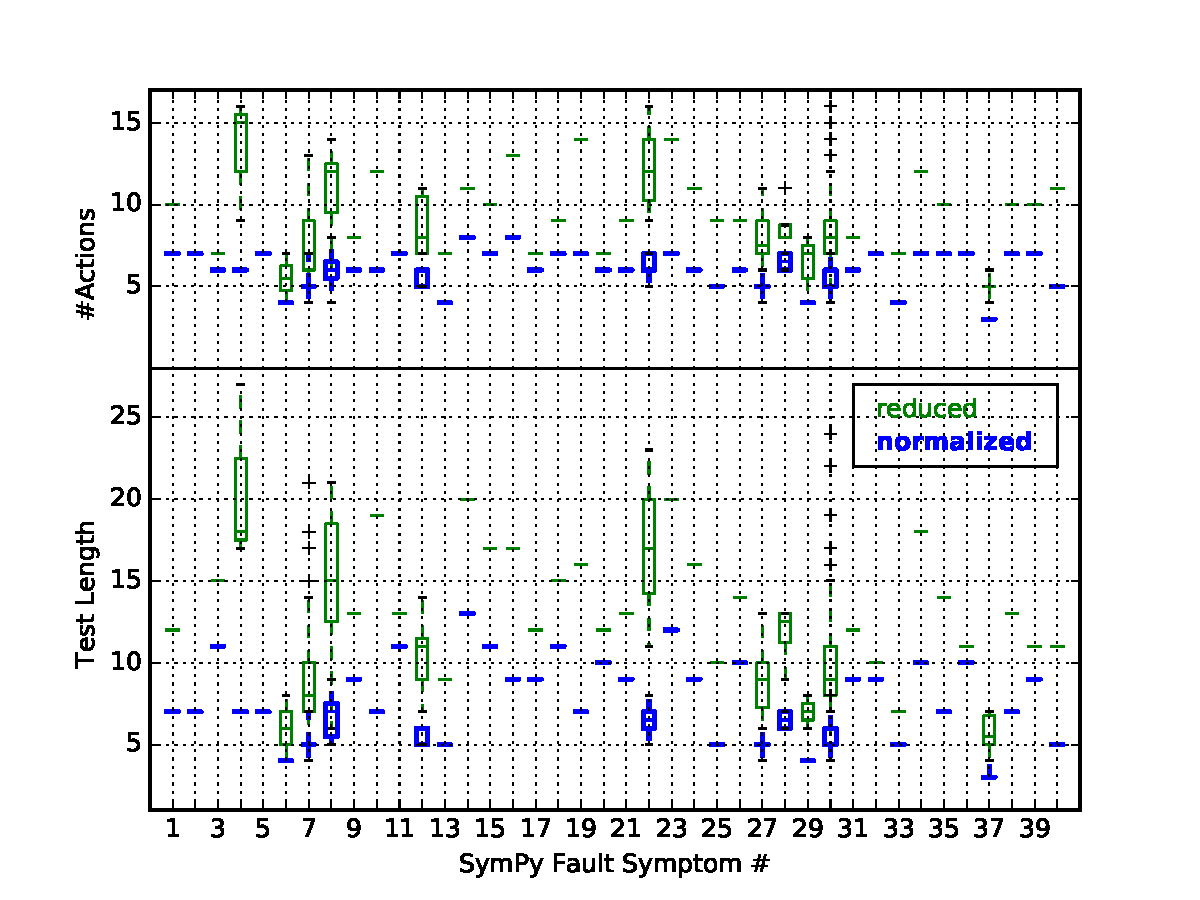
\includegraphics[width=\columnwidth]{sympyd}
\caption{Effects of normalization on SymPy tests.}
\label{lengthandactions}
\end{figure}

SymPy \cite{SymPy} is a widely used open source pure Python library
for symbolic mathematics.  SymPy is used by several other projects,
has over 400 contributors, over 25,000 commits to date, and over
225KLOC.  The TSTL tester for SymPy focuses on core expressions and
algebraic simplification, and covers about 15KLOC and 21,000 branches of
the system.  Testing this core resulted in discovery of a number
of faults in SymPy, detected by assertion violations or uncaught (and
not expected) exceptions.  Some of these have been reported to the project;
however, since SymPy currently has 2,128 open issues, with one opened
approximately each day, only one has (at this point) been fixed.  If we assume that
each different assertion violation or exception message indicates a
different underlying fault, SymPy provides us with a set of 40
complex, hard-to-understand real faults for evaluating normalization.
While we expect that this is an over-approximation of the actual
number of distinct faults, inspection of the tests and the covered
code suggests it is not far from the actual number.  Because we used a
(we believe)
non-lossy fault identification method (the exact failure symptom), our
SymPy results are relatively useless for {\bf RQ2}, but they answer {\bf RQ1}, {\bf RQ3}, and {\bf RQ4} for a large, realistic
system and real faults.

We generated, normalized, and reduced tests until we had 500 tests,
exhibiting all 40 fault signatures.    Some SymPy faults (not
included in our count of 40 tests) cause infinite loops, stopping
reduction or normalization. Of 570 failures, 549 reduced
and 500 both reduced and normalized.

{\bf RQ1:} Reduction alone did not reduce the number of distinct failing tests at
all.  Normalization reduced the total number of distinct
failing tests to 114.  There were
12.5 mean different failing tests, per fault, for both unreduced and
reduced tests, and only 3.15 mean failing tests per fault for
normalized tests.  This difference was significant, with $p=0.003$.
Normalization reduced the number of tests to
examine for 11 of the 13 faults with more than one failure; in 2 cases, the normalization was perfect (one failure).

{\bf RQ3:} The mean time for reduction was 104.45 seconds, with a
median of 19.70 seconds.  The mean time for normalization was
594 additional seconds, with a median of 260.214 seconds.  The
difference was significant, with $p\leq1\times10^{-80}$.

{\bf RQ4:} The mean length of unreduced tests was 44.664 steps, with a median
of 40.5 steps.  For reduced tests, this shrank to a mean of
9.984 and a median of 9.0 steps.  Normalized tests had mean length of
5.48 steps and median of 5.0 steps.  SymPy failures show
that normalization reduces not only the length of tests, but the number of
actions (roughly speaking, different API/method calls/functions) that must be considered for debugging:  reduced tests included
8.116 mean different actions, but normalized tests only 5.282
mean different actions.  These differences were all statistically
significant with $p\leq1\times10^{-76}$.  
Normalization made it possible to completely ignore a large number of
SymPy functions for debugging purposes.  The unreduced and reduced
tests included all 50 SymPy functions tested.  The normalized tests,
however, included only 32 of these, and enabled us to ignore such
complex code as trigonometric expansion and simplification, power expansion,
logarithmic combination, and even generalized expansion.  Figure
\ref{lengthandactions} graphically shows the impact of normalization
on length and number of functions covered by reduced tests.  The lower
part of the figure shows changes in test length, and the upper part
shows, for the same fault, the change in number of different actions.
The green boxplots show reduced tests, while the emphasized blue
boxplots show normalized tests.  It is clear that normalization not
only has a significant effect on average, but has a large benefit for
most individual faults.  The reduction in tests to examine
is also shown, indirectly, by the fact that the ``boxes'' for
normalized data are often simply lines because the tests are similar or identical.

\subsubsection{SortedContainers}

SortedContainers \cite{SortedContainers} is a popular Python library
of about 2KLOC, that provides pure Python sorted containers that are as fast as C
extension containers.  We have reported 3 bugs in SortedContainers
(all quickly corrected).  One of these bugs causes an infinite loop,
making it difficult to reduce or normalize.  We therefore only present
results for the other two faults reported.  We
generated 168 failing tests, all distinct, exhibiting both reported
faults, over 15 hours of testing. All failures reduced and normalized.
{\bf RQ1-RQ3:} Reduction did not reduce
the number of failures, but did reduce mean test length from
80.8 to 13.2 steps (median from 85.0 to 12.5), and mean number of
different actions per test from 14.4 to 7.4 (median from 14.0 to 8.0).
Normalization was perfect:  all tests normalized to two canonical
tests, one per fault, both with only 6 steps and 5
distinct actions --- a $>$ 50\% reduction in size beyond delta-debugging.  Changes were significant with
$p\leq1.0\times10^{-24}$.  There were 95 total
different actions in tests before reduction, 27 in tests after
reduction, and only 7 between the two normalized tests.  {\bf RQ4:} Reduction took a mean of 0.09 seconds, normalization a mean of 134.1
seconds (median 0.06 vs. 57.0) (significant, $p\leq1\times10^{-28}$).  

Table \ref{sumreduction} summarizes mean results for SymPy and
SortedContainers, our primary results for large numbers of failing
tests for real faults of complex programs where normalization is
perhaps as useful for additional reduction beyond delta-debugging as
it is for reducing the number of tests to examine.

\subsubsection{NumPy}

\begin{comment}
\begin{figure}[t]
{\scriptsize
\begin{code}
 dim1 = 1                                       \# STEP 0
 shape2 = (dim1, dim1, dim1)                    \# STEP 1
 array1 = np.ones(shape2)                       \# STEP 2
 array0 = array1 * array1                       \# STEP 3
 array1 = array1 + array1                       \# STEP 4
 array4 = array0 + array1                       \# STEP 5
 array0 = np.reshape(array4,shape2)             \# STEP 6 
 array3 = array1 * array4                       \# STEP 7
 array2 = np.ravel(array4)                      \# STEP 8
 array5 = array2 - array3                       \# STEP 9 
 array4 = array5 * array2                       \# STEP 10
 array1 = np.unique(array0)                     \# STEP 11
 array5 = array5 * array3                       \# STEP 12
 array0 = array1 * array5                       \# STEP 13
 array5 = np.unique(array0)                     \# STEP 14
 array1 = array4 - array2                       \# STEP 15
 array2 = array0.flatten()                      \# STEP 16
 array0 = array5 + array5                       \# STEP 17
 array5 = array5 + array2                       \# STEP 18
 array2 = array0 * array2                       \# STEP 19
 np.copyto(array5,array2)                       \# STEP 20
 array2 = array2 * array5                       \# STEP 21
 array3 = array0 * array2                       \# STEP 22
 array0 = array3 - array1                       \# STEP 23
 array4 = array3 * array0                       \# STEP 24
 array1 = array5 + array4                       \# STEP 25
 array5 = array0 * array1                       \# STEP 26
 array0 = array5 - array1                       \# STEP 27
 array4 = array0 * array3                       \# STEP 28
 array3 = array4 * array0                       \# STEP 29
 array1 = array5 + array3                       \# STEP 30
 array0 = array2 + array1                       \# STEP 31
 array5 = array5 - array0                       \# STEP 32
 array5 = array3 * array5                       \# STEP 33
 array0 = array1 + array5                       \# STEP 34
 array2 = array3 - array0                       \# STEP 35
 array4 = array2 * array1                       \# STEP 36
 array3 = array4 * array2                       \# STEP 37
 array2 = array0 - array0                       \# STEP 38
 np.copyto(array1,array3)                       \# STEP 39
 array4 = array2.flatten()                      \# STEP 40
 array1 = array1 * array4                       \# STEP 41
 assert (np.array\_equal(array1,array1))
\end{code}
}
\caption{Reduced () ``failing'' test for NumPy.}
\label{numpyorig}
\end{figure}
\end{comment}

Our final two case studies provide little information on {\bf RQ1} and
{\bf RQ2}; for these SUTs, failure rates are low enough or test
reduction runtimes high enough that each failure is usually dealt with
one-by-one.  However, the value of normalization and generalization
for further reduction ({\bf RQ4}) and aiding in understanding tests is effectively shown by these complex programs.  They also provide
results for {\bf RQ3} when even test \emph{reduction} is expensive.
NumPy \cite{NumPy} is a widely used Python library that
supports large, multi-dimensional matrices and provides a huge library
of mathematical functions.  The SciPy library for scientific
computing builds on NumPy.  Developing tests for NumPy is challenging,
because none of the authors are experts in numeric computation, and
the specification of correct behavior is often somewhat subtle.  As an
example, consider the test in Figure \ref{numpynormgen}.  Prior to
normalization, understanding why the test leads to a violation of
self-equality for an array is difficult: the reduced-only test has 42
steps and includes not only array multiplication and addition, but
subtraction, array copying, reshaping, flattening,  filtering by
unique elements, and raveling.  After
normalization, it is much clearer what is happening: 1) {\tt array0}
contains {\tt NaN} and 2) this is correct behavior (the array
\emph{should} contain {\tt NaN}).  The greater length and much larger
number of operations involved in the original reduced test
obscures this critical point.  In NumPy, array equality does not hold
for objects containing {\tt NaN}, so the assertion must be modified.
As far as we know, normalization transforms all instances of this
fault into this canonical test, but our data is insufficient to make a definite claim.

Other, more complex, failures have also made it clear that
normalization is useful for additional test length reduction for
NumPy, and that generalization makes any surprising restrictions on
test values clear.  For NumPy tests, normalization takes much longer
than reduction, in part due to the expense of operations on large
arrays.  For almost all tests, the mean time to reduce tests
is about 4-5 seconds, and the time for normalization is between 712
and 774 seconds.   Generalization takes
between 52 and 59 seconds in these cases.  The exception was a test of 45,206 steps (!)  leading to a memory exhaustion error and
crash.  This was reduced (over nearly a day) to a test
with 10 steps, which then normalized (in only 2 hours) to a test
with 8 steps.  The normalized test involved no operations other than array
initialization, array flattening, and array
addition.  The reduced test involved larger array dimensions, array
multiplication, and array subtraction, as well.  
%This is the only case in
%which we have seen normalization time lower than reduction time,
%without assistance from the cache.



\begin{figure}
{\scriptsize
\begin{code}
dim0 = 1                            \textcolor{black!60}{\# STEP 0}
\textcolor{black!60}{\#  or dim0 = 10 }
shape0 = (dim0)                     \textcolor{black!60}{\# STEP 1}
\textcolor{black!60}{\#  or shape0 = (dim0, dim0) }
\textcolor{black!60}{\#  or shape0 = (dim0, dim0, dim0) }
array0 = np.ones(shape0)            \textcolor{black!60}{\# STEP 2}
array0 = array0 + array0            \textcolor{black!60}{\# STEP 3}
array0 = array0 + array0            \textcolor{black!60}{\# STEP 4}
\textcolor{black!60}{\#  or array0 = array0 * array0 }
array0 = array0 * array0            \textcolor{black!60}{\# STEP 5}
array0 = array0 * array0            \textcolor{black!60}{\# STEP 6}
array0 = array0 * array0            \textcolor{black!60}{\# STEP 7}
array0 = array0 * array0            \textcolor{black!60}{\# STEP 8}
array0 = array0 * array0            \textcolor{black!60}{\# STEP 9}
array0 = array0 * array0            \textcolor{black!60}{\# STEP 10}
array0 = array0 * array0            \textcolor{black!60}{\# STEP 11}
array0 = array0 * array0            \textcolor{black!60}{\# STEP 12}
array0 = array0 * array0            \textcolor{black!60}{\# STEP 13}
array0 = array0 - array0            \textcolor{black!60}{\# STEP 14}
assert (np.array\_equal(array0,array0))
\end{code}
}
\caption{Normalized and generalized NumPy test.}
\label{numpynormgen}
\end{figure}

\subsubsection{Esri ArcPy}

Esri is the single
largest Geographic Information System (GIS) software vendor.  Esri's ArcGIS tools are widely
used for GIS analysis.  Automation is essential for complex GIS analysis and
data management, and Esri has long provided tools
for programming GIS software systems.  One such tool
is a Python site-package, ArcPy \cite{ArcPy}.  ArcPy is a complex library,
with dozens of classes and hundreds of functions.  Most of the code involved in ArcPy
functionality is the C++ source for ArcGIS itself (which is not
available), but the released Python interface code alone is over 50KLOC.
We have  discovered and reported six crash-inducing faults in
ArcPy/ArcGIS.  
%It is critical to understand these
%faults and the behaviors that trigger them to modify the harness to
%avoid triggering these faults, while restricting other testing as
%little as possible.

%There is no space in this paper to elaborate on the details of this
%large test effort (which has introduced numerous additional features
%and modes to TSTL), but normalization and generalization have been
%very useful in this process.  

Figures \ref{esriorig} and
\ref{esrinormgen} show one crash-inducing test, after initial
delta-debugging (from over 2,000 test steps) (Figure \ref{esriorig})
and after normalization and generalization (Figure \ref{esrinormgen}).
In this setting normalization has contributed a significant amount of
additional reduction over delta-debugging.  For the crash fault shown
in this paper, normalization reduced the length from 19 steps to 11
steps.  For three other crashes, normalization reduced the tests
from 18 to 14 steps, from 27 to 20 steps, and from 20 to 16 steps. One crash fault only reduced from 10 steps to 9 steps, but the
omission was informative.  None of the ArcPy faults experienced slippage --- the normalized
test was always clearly the same fault as the reduced test.
 The cost of normalization is high --- in
our runs, it has taken from 17,340 seconds up to 24,769 seconds.
However, in this setting even delta-debugging is extremely expensive
--- the cost of reduction alone has ranged from 7,930 seconds to 8,688
seconds.  Generalization has taken between 3,203 and
 11,149 seconds.  These high costs are due to the need to run
tests in a sandbox environment to avoid killing the testing
process, and the runtime of complex GIS analyses.
Even under these circumstances, reducing, normalizing, and
generalizing tests has been a more effective use of human time than
trying to understand the faults without help.  For example, in
the test shown in this paper, it was important to understand that
the SQL query and selection type are not essential, but using a
freshly created layer will not result in a crash: the problem appears
to be that ArcGIS (or ArcPy) does not invalidate layers built from a
feature class when that feature class is deleted.  In this
  instance, a generalization (the fresh values generalization in
  particular) is informative by its absence: we know that it was attempted, but prevented
  failure.  The reduced, non-normalized test (Figure \ref{esriorig})
makes this far less clear, as the use of {\tt CopyFeatures} and the
multiplicity of shapefiles involved disguises the essence of the
problem.  

We are also preparing a test suite that covers as much as
possible of the Python source in the latest version of ArcPy
and records the values returned.  For future versions of ArcPy, a ``semantic diff'' based on these calls
can be produced, allowing developers to see how API usage changes with
new releases.  The tests in the suite are
normalized and generalized (based on code coverage and output, not
failure --- these tests all pass) to make them easy to understand, and show
which parameter combinations do not change results.


\begin{comment}
Normalization and generalization are also being used to prepare an
API-behavior regression suite for ArcPy.  One of the challenges of
using a large API like ArcPy is that behavior of the system can change
from version to version.  In some cases this is due to new faults, or
fixed faults, but in other cases there is an undocumented usage change.  To assist ArcPy
developers, we are preparing a test suite that covers as much as
possible of the Python source in the latest version of ArcPy
and records the values returned.  For future versions of ArcPy, a ``semantic diff'' based on these calls
can be produced.  The tests in the suite are
normalized and generalized to help users understand API usage
consequences, since Esri examples are limited to simple parameter
combinations, and many illegal combinations are not specified.
\end{comment}

\begin{figure}[t]
{\scriptsize 
\begin{code}
shapefile2 = "C:\\arctmp\\new3.shp"                               \# STEP 0 
shapefile1 = "C:\\arctmp\\new3.shp"                               \# STEP 1
featureclass2 = shapefile2                                      \# STEP 2
featureclass0 = shapefile1                                      \# STEP 3
shapefilelist2 = glob.glob("C:\\Arctmp\\*.shp")                   \# STEP 4
fieldname0 = "newf3"                                            \# STEP 5
shapefile1 = shapefilelist2 [0]                                 \# STEP 6
featureclass1 = shapefile1                                      \# STEP 7
arcpy.CopyFeatures\_management(featureclass1,featureclass2)     \# STEP 8
op1 = ">"                                                       \# STEP 9
newlayer2 = "l2"                                                  \# STEP 10
val1 = "100"                                                      \# STEP 11
selectiontype2 = "SWITCH\_SELECTION"                               \# STEP 12
fieldname1 = "newf1"                                              \# STEP 13
arcpy.MakeFeatureLayer\_management(featureclass0, newlayer2)   \# STEP 14
arcpy.SelectLayerByAttribute\_management
   (newlayer2,selectiontype2,' "'+fieldname0+'" '+op1+val1)   \# STEP 15
op0 = ">"                                                        \# STEP 16
arcpy.Delete\_management(featureclass2)                           \# STEP 17
arcpy.SelectLayerByAttribute\_management
   (newlayer2,selectiontype2, ' "'+fieldname1+'" '+op0+val1) \# STEP 18
\end{code}
}
\caption{Test with reduction-only for ArcPy.}
%\vspace{-0.33in}
\label{esriorig}
\end{figure}

\begin{figure}[t]
{\scriptsize 
\begin{code}
shapefilelist0 = glob.glob("C:\\Arctmp\\*.shp")                 \textcolor{black!60}{\# STEP 0}
\textcolor{black!60}{\#[}
shapefile0 = shapefilelist0 [0]                                   \textcolor{black!60}{\# STEP 1}
newlayer0 = "l1"                                                  \textcolor{black!60}{\# STEP 2}
\textcolor{black!60}{\#  or newlayer0 = "l2" }
\textcolor{black!60}{\#  or newlayer0 = "l3" }
\textcolor{black!60}{\#  swaps with steps 3 4 5 6 7}
\textcolor{black!60}{\#] (steps in [] can be in any order)}
\textcolor{black!60}{\#[}
featureclass0 = shapefile0                                        \textcolor{black!60}{\# STEP 3}
\textcolor{black!60}{\#  swaps with step 2}
fieldname0 = "newf1"                                              \textcolor{black!60}{\# STEP 4}
\textcolor{black!60}{\#  or fieldname0 = "newf2" }
\textcolor{black!60}{\#  or fieldname0 = "newf3" }
\textcolor{black!60}{\#  swaps with steps 2 8}
selectiontype0 = "SWITCH\_SELECTION"                               \textcolor{black!60}{\# STEP 5}
\textcolor{black!60}{\#  or selectiontype0 = "NEW\_SELECTION" }
\textcolor{black!60}{\#  or selectiontype0 = "ADD\_TO\_SELECTION" }
\textcolor{black!60}{\#  or selectiontype0 = "REMOVE\_FROM\_SELECTION"}
\textcolor{black!60}{\#  or selectiontype0 = "SUBSET\_SELECTION"}
\textcolor{black!60}{\#  or selectiontype0 = "CLEAR\_SELECTION"   }
\textcolor{black!60}{\#  swaps with steps 2 8}
op0 = ">"                                                         \textcolor{black!60}{\# STEP 6}
\textcolor{black!60}{\#  or op0 = "<" }
\textcolor{black!60}{\#  swaps with steps 2 8}
val0 = "100"                                                      \textcolor{black!60}{\# STEP 7}
\textcolor{black!60}{\#  or val0 = "1000" }
\textcolor{black!60}{\#  swaps with steps 2 8}
\textcolor{black!60}{\#] (steps in [] can be in any order)}
arcpy.MakeFeatureLayer\_management(featureclass0, newlayer0)    \textcolor{black!60}{\# STEP 8}
\textcolor{black!60}{\#  swaps with steps 4 5 6 7}
arcpy.SelectLayerByAttribute\_management
   (newlayer0,selectiontype0,' "'+fieldname0+'" '+op0+val0)    \textcolor{black!60}{\# STEP 9}
arcpy.Delete\_management(featureclass0)                             \textcolor{black!60}{\# STEP 10}
arcpy.SelectLayerByAttribute\_management
   (newlayer0,selectiontype0,' "'+ fieldname0+'" '+op0+val0) \textcolor{black!60}{\# STEP 11}
\end{code}
}
\caption{Normalized and generalized ArcPy test.}
\label{esrinormgen}
\end{figure}


\section{Related Work}

This work builds on the idea behind delta-debugging \cite{DD}: tests should not contain extraneous information that is not needed to
reproduce failure (or some other behavior \cite{icst2014,stvrcausereduce}).  Delta-debugging and slicing
\cite{TCminim} are limited, generally, to producing subsets of the
original test, not modifying parts of the test to obtain further
simplicity.  We extend this concept by also allowing modification or
re-ordering, which also allows further length reduction.

%Some earlier work in bounded model checking modified counterexamples to use
%numerically smaller values \cite{MakeMost} but otherwise did not aim
%to simplify or normalize failures.

Normalization is in part motivated by the fuzzer taming \cite{PLDI13}
problem: determining how many distinct faults are present in a large
set of failing tests.  This is a key problem in practical
application of automated testing.  Previous work on fuzzer taming
\cite{PLDI13} used delta-debugging to reduce some tests to
syntactic duplicates.

Zhang \cite{SaiSimple} proposed an alternative approach to semantic
test simplification that, like our approach, is able to modify, rather
than simply remove, portions of a test.  However, because Zhang
operates directly over a fragment of the Java language, rather than
using an abstraction of test actions allowed, the set of rewrite
operations performed is highly restricted: no new methods can be
invoked, statements cannot be re-ordered, and no new values are used.
These restrictions limit the approach's ability to simplify tests and
make it inappropriate for  normalization, as opposed to simplification.  The approach also performs little
syntactic normalization: e.g., it does not even force a test to use
fixed variable names when variable name is irrelevant.  CReduce
\cite{CReduce} performs some simple normalization as part of a complex
test reduction scheme for C code, and the peephole-rewrite scheme
used in CReduce is also an inspiration for the approach taken by our
normalizer.

Work on automatically producing readable tests \cite{Guava,Readable} is also
related, in that it aims to ``simplify'' tests.  Readable tests are
intended to assist debugging by humans, while our
normalization and generalization aims to increase the information
density of a test, further reduce length, and address the fuzzer taming problem.  The approaches are
orthogonal and could likely be profitably combined: users might be
best served by normalized, generalized tests modified to improve readability.

The most closely related work to our generalization efforts is Pike's
SmartCheck \cite{SmartCheck}.  SmartCheck targets algebraic data in
Haskell, and offers an interesting alternative approach to reduction
and generalization.  Test generalization is also akin to dynamic invariant generation,
in that it informs the user of invariants over a series of test
executions \cite{Daikon}.  The only other work we are aware of that is
similar to generalization concerns essential and accidental aspects of
model checking counterexamples \cite{FreeWill,MakeMost,SPIN03}.  



\section{Conclusions and Future Work}

This paper presents a set of tools, part of the TSTL \cite{tstlsttt}
testing language and tool suite, for letting users make the most of the
tests the tool generates.  In addition to standard
replay, regression, and minimization, TSTL implements some powerful
new techniques from the recent literature for manipulating tests
\cite{OneTest,slippage}.

As future work, we plan to continue to develop TSTL's tools for
working with tests.  Some improvments are simple:  for instance, the TSTL
random tester currently provides simple fault localization over the
tests generated during a run (if there are any failures)
\cite{Tarantula}.  However, the regression tool does not yet provide
the same functionality for a suite of stored tests.  More importantly,
we plan to continue to use TSTL as a platform for experimenting with
and making available novel methods for making use of automatically
generated tests, including methods for composing and de-composing
tests and generating information from tests that can be used to guide
future testing.

\bibliographystyle{IEEEtran}
% argument is your BibTeX string definitions and bibliography database(s)

\def\IEEEbibitemsep{0.6pt plus 0.9pt}

\bibliography{bibliography}

\end{document}